
Abbiamo definito un problema di classificazione multiclasse.
Essendo un problema multiclasse è necessario utilizzare un metodo tipo one-vs-all oppure all-vs-all.
In questo caso utilizziamo un classificatore lineare con un metodo all-vs-all, in cui ogni classe è paragonata a tutte le altre ad ogni nuova iterazione dell'algoritmo.

Utilizzo come parametro di regolarizzazione lambda.
Per ottenere la soluzione ottima dividiamo il dataset in due insiemi: un learning set, corrispondente al $70/$ dei dati inizali e un validation set per poter calcolare l'errore commesso dal nostro modello ed eseguiamo un ciclo su diversi valori di lambda in modo da individuare il valore migliore.

Per mediare il risultato e minimizzare l'influenza della varianza ripetiamo questo procediamo un numero k di volte, con k uguale a 30 ad esempio.

We have defined a multiclass classification problem.
Being a multiclass problem it is necessary to use a one-vs-all or all-vs-all method.
In this case we use a linear classifier with an all-vs-all method, in which each class is compared to all the others with each new iteration of the algorithm.

Use as a $\lambda$ regularization parameter.
To get the best solution we divide the dataset into two sets: a learning set, corresponding to the $ 70 / $ of the initial data and a validation set in order to calculate the error committed by our model and run a cycle on different lambda values in order to identify the best value.

To mediate the result and minimize the influence of variance we repeat this we proceed a number k of times, with k equal to 30 for example.
\begin{figure}[h]
	\centering
	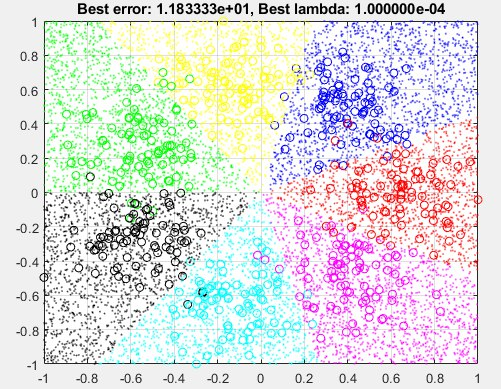
\includegraphics[width=0.5\textwidth]{i1.png}
	\caption{Regression Function}
	\label{fig:regression function}
\end{figure}


